\documentclass{article}
\usepackage{setspace}
\usepackage{sectsty}
\usepackage{indentfirst}
\usepackage[left=2.5cm, right=2.5cm, top=1.5cm, bottom=1.5cm]{geometry}
\usepackage{hyperref}
\usepackage{pgfplots}
\usepgfplotslibrary{dateplot}
\hypersetup{
    colorlinks=true,
    linkcolor=blue,
    filecolor=magenta,      
    urlcolor=blue,
}


\title{O impacto da pandemia na economia da Airbnb}
\author{Lucas Oliveira Campos\and Bruno Augusto Teixeira\and Esdras Silva de Lima Junior\and Davi Henrique Souto Almeida
}
\date{07/04/2023}
\renewcommand{\abstractname}{Resumo}
\begin{document}

\maketitle

\onehalfspacing
\section*{Resumo}
O modelo de negócio da Airbnb revolucionou a indústria de hospedagem, conectando viajantes a anfitriões que desejam alugar suas propriedades. A empresa adotou um modelo de marketplace P2P, onde cobra uma taxa de reserva dos viajantes e uma taxa dos anfitriões pelas reservas bem-sucedidas. Com sua plataforma, o Airbnb oferece uma experiência diferenciada aos clientes, diversidade de opções de hospedagem e uma oportunidade de renda extra para os locatários.

A pandemia da COVID-19 teve um impacto significativo na Airbnb e no mercado de turismo em geral. As cotações da empresa apresentaram flutuações, refletindo os desafios enfrentados durante a pandemia. Houve uma queda acentuada nas cotações em 2022, seguida por uma recuperação gradual em 2023, mas ainda abaixo dos níveis pré-pandemia. A Airbnb enfrentou uma diminuição nas reservas e na receita no início da pandemia, mas começou a se recuperar com a crescente demanda por viagens domésticas e locais de férias isolados e seguros.

Para enfrentar os desafios da pandemia, a Airbnb implementou estratégias como o foco em viagens domésticas e experiências locais, além de medidas de segurança e higiene. Essas ações visam atender às necessidades e preocupações dos consumidores em um contexto de pandemia e contribuir para a manutenção da posição da Airbnb no mercado.

Em resumo, a Airbnb revolucionou o setor de hospedagem com seu modelo de negócio P2P e uma proposta de valor única. A empresa enfrentou desafios durante a pandemia, mas está se adaptando e implementando estratégias para se manter resiliente e continuar atendendo às demandas dos consumidores. Com sua posição de destaque no mercado e capacidade de inovação, a Airbnb está bem posicionada para enfrentar os desafios futuros e aproveitar as oportunidades no setor de hospedagem.
\vspace{1cm}
\onehalfspacing 

\section*{Palavras-chave:}
Airbnb, Coronavírus, Covid-19, Economia, Cotações, Modelo de negócio, Hospedagem, Marketplace P2P, Pandemia, Flutuações, Recuperação, Viagens domésticas, Experiências locais, Medidas de segurança e higiene, Adaptação, Demandas dos consumidores, Posição de destaque, Capacidade de inovação, Desafios futuros, Oportunidades.
\vspace{1cm}
\onehalfspacing


\section*{Abstract}
The Airbnb business model has revolutionized the hospitality industry by connecting travelers with hosts who want to rent out their properties. Adopting a peer-to-peer (P2P) marketplace model, Airbnb charges a booking fee from travelers and a commission fee from hosts for successful reservations. Through its platform, Airbnb offers a differentiated customer experience, a wide range of accommodation options, and an opportunity for hosts to earn extra income.

The COVID-19 pandemic had a significant impact on Airbnb and the tourism market in general. The company's stock prices fluctuated, reflecting the challenges faced during the pandemic. There was a sharp decline in stock prices in 2022, followed by a gradual recovery in 2023, but still below pre-pandemic levels. Airbnb experienced a decline in bookings and revenue at the onset of the pandemic but began to recover with the increasing demand for domestic travel and secluded, safe vacation destinations.

To address the challenges of the pandemic, Airbnb implemented strategies such as focusing on domestic travel and local experiences, as well as implementing safety and hygiene measures. These actions aim to meet consumer needs and concerns in the context of the pandemic and contribute to maintaining Airbnb's position in the market.

In summary, Airbnb has revolutionized the hospitality sector with its P2P business model and unique value proposition. The company faced challenges during the pandemic but is adapting and implementing strategies to remain resilient and meet consumer demands. With its prominent market position and capacity for innovation, Airbnb is well-positioned to tackle future challenges and capitalize on opportunities in the hospitality industry.
\vspace{1cm}
\onehalfspacing

\section*{Keywords:}
Airbnb, Business model, Peer-to-peer marketplace, COVID-19, Pandemic impact, Travel industry, Accommodation, Reservations, Revenue, Adaptation, Recovery, Domestic travel, Safety measures, Consumer demands, Market position, Innovation, Future challenges, Opportunities.
\vspace{1cm}
\onehalfspacing

\section*{Introdução}
\normalsize \onehalfspacing
%INTRODUÇÃO
A pandemia global causada pelo coronavírus afetou significativamente diversos setores da economia, incluindo o turismo e a hotelaria. Uma das empresas que sentiu o impacto da crise foi a Airbnb, que depende do fluxo constante de turistas para sua plataforma de hospedagem compartilhada. Com o surgimento da pandemia e as restrições de viagem impostas em muitos países, a demanda por hospedagem no Airbnb diminuiu drasticamente, afetando sua receita e, consequentemente, sua cotação na bolsa de valores.
\footnotetext{Universidade Nove de julho, São Paulo, Brasil.}

\newpage
\section*{Descrição do modelo de negócio da Airbnb}
O Airbnb é uma startup que revolucionou a forma como as pessoas se hospedam em suas viagens ao redor do mundo. Fundada em 2008 por Nathan Blecharczyk, Brian Chesky e Joe Gebbia, a empresa tinha como objetivo criar uma plataforma que tornasse mais fácil para os viajantes encontrarem hospedagem em casas, apartamentos e quartos, oferecidos por pessoas que tinham lugares extras para alugar. Usando o modelo de marketplace, o Airbnb conecta dois segmentos de clientes, aqueles que querem alugar e aqueles que têm algo para alugar. Com o tempo, a empresa se estabilizou e conseguiu escalar sua oferta de serviços, levantando milhões de dólares em investimentos.

O modelo adotado pelo Airbnb é conhecido como P2P (peer-to-peer), em referência aos sistemas P2P de compartilhamento de arquivos pela internet. O modelo evoluiu e atualmente a empresa cobra nas duas pontas, uma taxa de reserva dos viajantes (6-12\%) e uma taxa dos anfitriões pelas reservas bem sucedidas (3\%). A empresa oferece uma experiência diferenciada para os clientes, incluindo opções de locais diferentes, além de proporcionar uma renda extra para os locatários. A empresa também se preocupa com a segurança de quem aluga o seu local, oferecendo um seguro de até 50 mil dólares em casos de roubo e se adequando às legislações locais dos países em que atua. Além disso, o Airbnb teve um grande diferencial competitivo ao contratar fotógrafos profissionais para tirar as fotos das casas para os anúncios, tornando as fotos mais atraentes para os potenciais clientes. Todo esse conjunto de estratégias contribuiu para o sucesso da empresa e seu impacto na economia.
% -------------------------%
\section*{Impactos da pandemia}
A pandemia da COVID-19 afetou significativamente o mercado de turismo e hospedagem, incluindo a empresa Airbnb. Em 2019, antes da pandemia, as cotações da empresa estavam em cerca de 146.800. No entanto, com o surgimento da pandemia, as cotações da Airbnb começaram a flutuar e apresentaram uma queda acentuada em 2022, chegando a 85.500 em dezembro do mesmo ano. No entanto, em janeiro de 2023, as cotações da empresa subiram para 111.110, ainda abaixo do nível pré-pandemia.

É importante notar que as flutuações nas cotações da Airbnb não foram apenas causadas pela pandemia, mas também foram influenciadas por outros fatores, como o desempenho financeiro da empresa e a concorrência de outras empresas no setor de hospedagem. Além disso, a Airbnb relatou uma diminuição significativa no número de reservas e na receita durante o primeiro semestre de 2020. No entanto, a partir do segundo semestre do mesmo ano, a empresa apresentou uma recuperação gradual, impulsionada pela crescente demanda por viagens domésticas e locais de férias mais isolados e seguros.

Diante das incertezas causadas pela pandemia, a Airbnb tem implementado estratégias para enfrentar os desafios do mercado. Entre as iniciativas estão o aumento do foco em viagens domésticas e experiências locais, bem como a implementação de medidas de segurança e higiene em suas acomodações. Essas ações podem ajudar a Airbnb a manter sua posição no mercado e continuar se adaptando às mudanças no comportamento dos consumidores.
% -------------------------%
\section*{Protocolos de segurança adotados pelo Airbnb durante a pandemia de COVID-19: estratégias inovadoras para garantir o bem-estar dos usuários}

A pandemia de COVID-19 impactou o mundo inteiro, afetando tanto a saúde quanto a economia global. Com o setor de turismo sendo um dos mais afetados, o Airbnb, uma plataforma de compartilhamento de acomodações, desenvolveu em junho de 2020 o Protocolo Avançado de Higienização em 5 etapas, orientado por autoridades sanitárias e especialistas internacionais, para garantir a segurança e o bem-estar de seus usuários. O Protocolo inclui especificações sobre como higienizar todos os cômodos de uma casa e um selo para as acomodações, solicitado a todos os anfitriões. Essa iniciativa pioneira no setor demonstra o compromisso do Airbnb com a segurança e o bem-estar de seus usuários.

Além disso, a empresa proibiu festas e eventos em acomodações para evitar aglomerações e contribuir para estadias responsáveis. Tanto anfitriões quanto hóspedes são incentivados a seguir as orientações e boas práticas disponíveis no site da plataforma, como o uso de máscaras e a prática de distanciamento social. Em agosto de 2020, o Airbnb lançou o Canal de Apoio ao Vizinho, uma ferramenta para auxiliar as autoridades e comunidades locais e facilitar a comunicação de eventuais incidentes em reservas nas proximidades. Com essa atualização, a vizinhança terá um canal de acesso direto com o Airbnb 24 horas por dia, 7 dias por semana, tornando-se um importante meio de colaboração para uma estadia mais segura e responsável.

Essas estratégias adotadas pelo Airbnb para enfrentar a pandemia de COVID-19 demonstram o compromisso da empresa com a segurança e o bem-estar de seus usuários. Além disso, a iniciativa é um exemplo de como as empresas podem se adaptar e inovar em momentos de crise, buscando soluções que atendam às necessidades de seus clientes e da sociedade em geral. O Protocolo Avançado de Higienização em 5 etapas, a proibição de festas e eventos em acomodações e o Canal de Apoio ao Vizinho são algumas das estratégias implementadas pelo Airbnb para enfrentar a pandemia de COVID-19. Essas iniciativas foram pioneiras no setor de compartilhamento de acomodações e demonstram o compromisso da empresa com a segurança e o bem-estar de seus usuários.
% -------------------------%
\section*{Estratégias de Limpeza da Airbnb para Garantir a Segurança dos Hóspedes e Anfitriões durante a Pandemia}
A limpeza é uma das estratégias mais importantes que a Airbnb implementou durante a pandemia para garantir a segurança dos seus hóspedes e anfitriões. A empresa divulgou um guia de limpeza rápida que detalha cinco etapas importantes para garantir a higienização adequada dos espaços.

A primeira etapa é a preparação do ambiente. É necessário abrir as janelas para permitir a circulação de ar, retirar o lixo e colocar novos sacos, além de lavar as roupas de cama e limpar a louça.

A segunda etapa é a limpeza propriamente dita. É importante varrer ou aspirar todos os pisos, limpar todas as superfícies impermeáveis com água e sabão e seguir as instruções do fabricante para limpar partes específicas de superfícies permeáveis. É recomendado evitar tocar o rosto durante a limpeza.

A terceira etapa é a higienização. Após limpar as superfícies, é importante aplicar um desinfetante aprovado e deixá-lo agir pelo tempo especificado no rótulo do fabricante. É recomendado usar um pano umedecido por superfície.

A quarta etapa é a verificação. É importante conferir se todas as superfícies tocadas com frequência foram higienizadas e checar as orientações para cada cômodo. Além disso, é importante verificar se há problemas de manutenção e se é necessário reabastecer produtos de limpeza ou desinfetantes.

A quinta e última etapa é a arrumação final. É necessário lavar as mãos e colocar luvas limpas antes de repor os suprimentos dos hóspedes, toalhas ou roupas de cama. É importante desinfetar a maçaneta e fechar a porta, não voltando ao espaço após higienizá-lo. Os materiais de limpeza e equipamentos de proteção devem ser eliminados ou lavados com segurança. Para os hóspedes, é recomendado preparar um kit de limpeza com itens como toalhas de papel, desinfetantes e sabonete extra para as mãos.

Essas cinco etapas, divulgadas pela Airbnb, são essenciais para garantir uma higienização adequada dos espaços e evitar a propagação do vírus. É importante segui-las rigorosamente para garantir a segurança dos hóspedes e anfitriões.

A Airbnb também destaca a importância de deixar um kit de limpeza para os hóspedes durante a estadia, com produtos confiáveis para os hóspedes manterem a limpeza e a higiene do ambiente durante a sua estadia. Isso pode ser informado no anúncio do imóvel e contribuir para a satisfação dos hóspedes.
% -------------------------%
\section*{Efeito da estratégia de limpeza da Airbnb}
De acordo com dados internos do Airbnb referentes às avaliações de hóspedes sobre a limpeza das estadias a partir de 1º de junho de 2021, 95\% das avaliações mostram que os hóspedes estão satisfeitos com a limpeza, obtendo uma pontuação de 4 ou 5 estrelas. Isso sugere que a estratégia de limpeza adotada pela Airbnb pode ter um impacto positivo na satisfação dos hóspedes e, consequentemente, na reputação da empresa. Além disso, uma pesquisa recente do Airbnb revelou que 87\% dos viajantes americanos consideram importante viajar com responsabilidade, o que sugere que a abordagem proativa da empresa em relação à saúde e segurança pode estar alinhada com as expectativas dos consumidores.
% -------------------------%
\vspace{3cm}
% -------------------------%
\section*{O canal de apoio ao vizinho do Airbnb: uma estratégia para promover estadias responsáveis}

Com a finalidade de promover estadias responsáveis e evitar aglomerações nas proximidades, o Airbnb lançou em agosto de 2020 uma política que proíbe festas e eventos nas propriedades listadas na plataforma. Como parte dessa iniciativa, a empresa lançou o Canal de Apoio ao Vizinho, que permite que a comunidade em geral reporte eventuais incidentes nas proximidades, como festas e eventos proibidos.

A atualização permite que a vizinhança tenha um canal de acesso direto com o Airbnb 24 horas por dia, 7 dias por semana, facilitando o relato de quaisquer descumprimentos às determinações das autoridades locais e aos termos de uso do Airbnb. O Brasil foi o primeiro país da América Latina a receber essa nova ferramenta, que já está em funcionamento em outros países, como Estados Unidos, Canadá, Reino Unido e Nova Zelândia.

Para reportar um incidente, a vizinhança pode acessar a página airbnb.com.br/vizinho e detalhar o caso por escrito, ou solicitar o apoio de um representante especializado, que dará retorno para atendimento por telefone. O Airbnb enfatiza que a segurança e o bem-estar dos anfitriões, hóspedes e da comunidade em geral são prioridades para a empresa, e que trabalha constantemente para prevenir incidentes na plataforma.

No caso de festas e eventos irregulares, os anfitriões e hóspedes envolvidos estão sujeitos às penalidades estabelecidas pelo Airbnb, que podem incluir remoção da plataforma, além de medidas legais cabíveis. A plataforma ressalta que adota diversas medidas para contribuir para a proteção da comunidade, como o Protocolo Avançado de Higienização, e que recomenda boas práticas também para hóspedes, com as quais é preciso se comprometer no momento da reserva, incluindo o uso de máscaras e a prática do distanciamento social.

Ao longo do período de um ano, entre 1º de julho de 2019 e 30 de junho de 2020, apenas 0,086\% das viagens tiveram algum incidente de segurança relatado por um anfitrião ou hóspede, globalmente. A plataforma conta com diversas ferramentas e processos de segurança para prevenir problemas desse tipo e para apoiar a comunidade caso eles aconteçam, incluindo perfis de anfitriões e hóspedes, sistemas para verificar a identidade de ambos, sistema de avaliações e comentários, pagamento seguro e 100\% rastreável via cartão de crédito, proteção contra danos à propriedade e central de ajuda 24 horas com atendimento em 11 idiomas, incluindo o português.
% -------------------------%
\section*{Efeitos da estratégia de apoio a vizinhança}

Os comentários fornecem um feedback positivo em relação à nova estratégia de apoio à vizinhança da Airbnb. Um usuário observa que essa ferramenta pode ajudar a solucionar problemas de barulho excessivo e festas em propriedades alugadas na plataforma. Além disso, outro usuário aponta que essa medida pode incentivar a comunicação entre os vizinhos e a celeridade nas informações em um momento em que a fluidez da informação é fundamental. Esses comentários mostram que a estratégia da Airbnb pode ter um efeito positivo na relação entre os usuários da plataforma e seus vizinhos.
% -------------------------%
\newpage
\section*{A volta por cima da Airbnb: como a empresa reergueu-se após a pandemia}
Com o impacto global da pandemia de COVID-19, muitas empresas do setor de turismo foram fortemente afetadas em 2020, incluindo a Airbnb. Em dezembro de 2020, a empresa teve uma cotação de mercado de apenas 146,8 dólares por ação. No entanto, a Airbnb tomou rapidamente medidas para se adaptar às mudanças na demanda do mercado e, em pouco tempo, conseguiu se recuperar e prosperar novamente.
A partir de janeiro de 2021, a Airbnb começou a ver um aumento constante em suas cotações de mercado. Em fevereiro, suas ações ultrapassaram a marca dos 200 dólares e continuaram a subir nos meses seguintes. A empresa manteve essa trajetória ascendente até o final de 2021, quando suas ações foram cotadas em cerca de 166,5 dólares.
\\
% -------------------------%
A partir de janeiro de 2021, a Airbnb começou a ver um aumento constante em suas cotações de mercado. Em fevereiro, suas ações ultrapassaram a marca dos 200 dólares e continuaram a subir nos meses seguintes. A empresa manteve essa trajetória ascendente até o final de 2021, quando suas ações foram cotadas em cerca de 166,5 dólares.

\begin{figure}[ht]
    \centering
    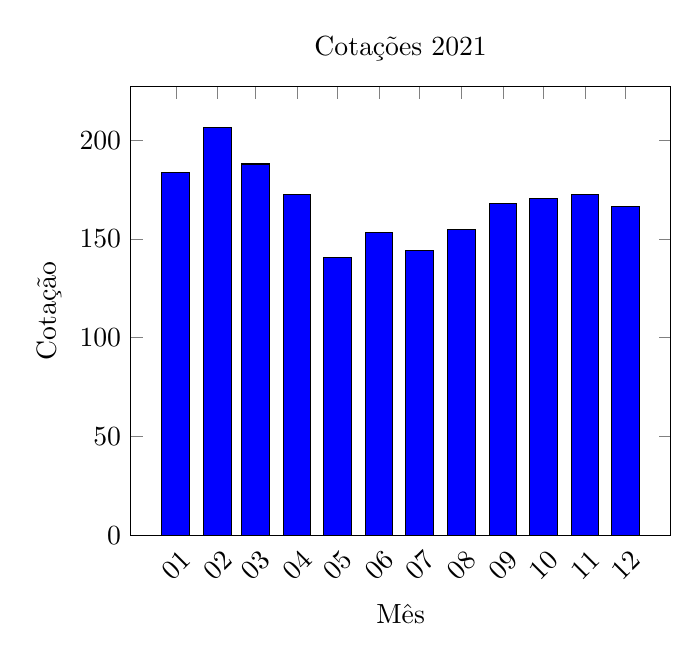
\begin{tikzpicture}
        \begin{axis}[
            title={Cotações 2021},
            xlabel={Mês},
            ylabel={Cotação},
            ymin=0,
            yticklabel style={
                /pgf/number format/fixed,
                /pgf/number format/precision=3
            },
            date coordinates in=x,
            xticklabel={\month},
            xtick={
                {2021-01-01},
                {2021-02-01},
                {2021-03-01},
                {2021-04-01},
                {2021-05-01},
                {2021-06-01},
                {2021-07-01},
                {2021-08-01},
                {2021-09-01},
                {2021-10-01},
                {2021-11-01},
                {2021-12-01}
            },
            xticklabel style={rotate=45, anchor=near xticklabel},
            ]
            \addplot[ybar,fill=blue] coordinates {
                (2021-01-01, 183.630)
                (2021-02-01, 206.350)
                (2021-03-01, 187.940)
                (2021-04-01, 172.710)
                (2021-05-01, 140.400)
                (2021-06-01, 153.140)
                (2021-07-01, 144.010)
                (2021-08-01, 154.990)
                (2021-09-01, 167.750)
                (2021-10-01, 170.660)
                (2021-11-01, 172.540)
                (2021-12-01, 166.490)};
    \end{axis}
    \end{tikzpicture}
    \end{figure}

Com base nos dados apresentados no gráfico, é possível observar que a Airbnb passou por um período de queda nas cotações de mercado no final de 2020, atingindo o valor mínimo de 146,8 dólares por ação em dezembro. Isso representa uma queda de aproximadamente 47,6\% em relação ao valor máximo do ano anterior. No entanto, a partir de janeiro de 2021, a empresa iniciou uma recuperação gradual, com um aumento constante nas cotações de mercado. Destaca-se uma forte valorização das ações em fevereiro, ultrapassando a marca dos 200 dólares, representando um aumento de cerca de 36,3\% em relação ao mês anterior. Apesar de algumas oscilações nos meses seguintes, a Airbnb manteve uma trajetória ascendente ao longo de 2021, alcançando um valor próximo a 166,5 dólares por ação no final do ano. Esse aumento representa cerca de 14,8\% em relação ao valor máximo de 2020. \\
Esses dados evidenciam a capacidade da empresa de se adaptar às mudanças na demanda do mercado e se recuperar após um período desafiador, o que pode servir como uma lição valiosa para outras empresas que enfrentam situações similares. Além disso, de acordo com informações da Forbes, a indústria de viagens está experimentando um aumento na demanda à medida que os casos de Covid-19 diminuem globalmente, e a Airbnb se destaca como um dos principais beneficiários dessa tendência, graças à preferência crescente dos consumidores por compartilhamento de casas e ao reconhecimento da marca da empresa. \\ 
É importante ressaltar que o preço das ações da Airbnb quase dobrou desde sua oferta pública inicial (IPO) em 2020, atingindo cerca de 125 dólares em 2021. Embora o preço das ações tenha sido volátil desde então, a natureza resiliente do modelo de negócios da Airbnb sugere que o preço das ações pode continuar em alta. \\ 
Após analisar as cotações de mercado da Airbnb em 2021, é interessante observar como a empresa lidou com as mudanças na demanda do mercado e como seus esforços para se adaptar resultaram em uma trajetória ascendente das cotações. No entanto, considerando a volatilidade das condições de mercado, é fundamental também avaliar o desempenho da Airbnb em 2022 para compreender se a empresa continua se adaptando bem às mudanças e mantendo-se em uma trajetória ascendente. O gráfico a seguir apresenta as cotações de mercado da Airbnb em 2022 até o momento, possibilitando uma análise mais aprofundada da performance recente da empresa. \\ \\
% -------------------------%
Com base nos dados apresentados, podemos observar no gráfico abaixo que as ações da Airbnb tiveram um início de ano relativamente estável, mantendo-se acima dos 150 dólares por ação nos primeiros meses de 2022. No entanto, a partir de maio, a cotação das ações da empresa começou a declinar significativamente, atingindo seu valor mínimo no final do ano.

\begin{figure}[ht]
    \centering
    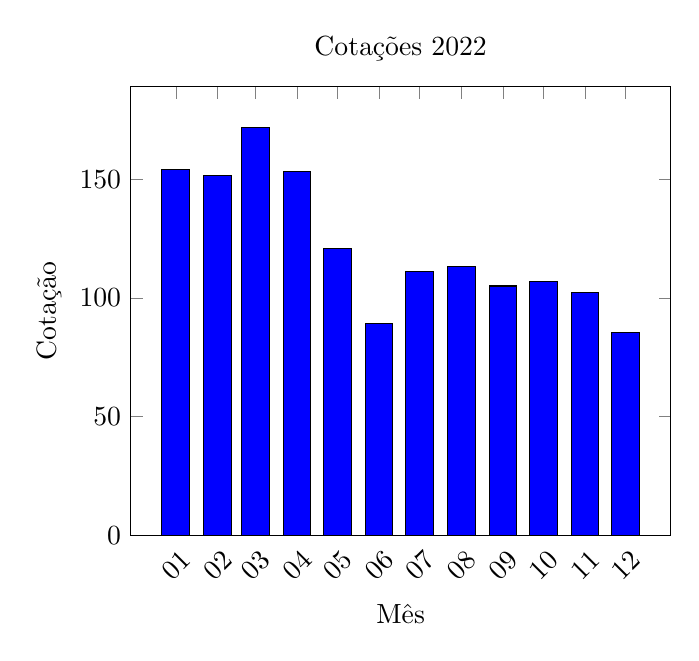
\begin{tikzpicture}
        \begin{axis}[
            title={Cotações 2022},
            xlabel={Mês},
            ylabel={Cotação},
            ymin=0,
            yticklabel style={
                /pgf/number format/fixed,
                /pgf/number format/precision=3
            },
            date coordinates in=x,
            xticklabel={\month},
            xtick={
                {2022-01-01},
                {2022-02-01},
                {2022-03-01},
                {2022-04-01},
                {2022-05-01},
                {2022-06-01},
                {2022-07-01},
                {2022-08-01},
                {2022-09-01},
                {2022-10-01},
                {2022-11-01},
                {2022-12-01}
            },
            xticklabel style={rotate=45, anchor=near xticklabel},
            ]
            \addplot[ybar,fill=blue] coordinates {
                (2022-01-01, 153.970)
                (2022-02-01, 151.490)
                (2022-03-01, 171.760)
                (2022-04-01, 153.210)
                (2022-05-01, 120.870)
                (2022-06-01, 89.080)
                (2022-07-01, 110.980)
                (2022-08-01, 113.120)
                (2022-09-01, 105.040)
                (2022-10-01, 106.910)
                (2022-11-01, 102.140)
                (2022-12-01, 85.50)};
    \end{axis}
    \end{tikzpicture}
    \end{figure}

Em maio, as ações da Airbnb caíram para cerca de 120,87 dólares por ação, representando uma queda de cerca de 21,3\% em relação ao valor máximo do ano anterior. A partir desse ponto, a queda continuou constantemente, com uma pequena recuperação em julho e agosto, mas voltando a cair em setembro e atingindo seu valor mínimo de 85,50 dólares por ação em dezembro.\\
Essa queda pode ser atribuída a uma série de fatores, como a pandemia em curso, que pode ter afetado a demanda por acomodações de viagem, bem como a competição cada vez maior no mercado de aluguel de curto prazo, que pode ter levado a uma diminuição no número de reservas feitas pelos usuários.\\
Uma análise mais detalhada dos dados pode revelar informações valiosas sobre o desempenho da Airbnb em 2022. Em janeiro e fevereiro, por exemplo, a empresa conseguiu manter um preço relativamente estável para suas ações, o que pode indicar que os investidores estavam confiantes em sua capacidade de se recuperar após um ano desafiador. \\
No entanto, a partir de maio, a queda nas cotações das ações da Airbnb pode ser vista como um sinal de que os investidores estavam começando a se preocupar com a resiliência da empresa diante de desafios contínuos, como a pandemia em curso.\\
Em resumo, embora a Airbnb tenha enfrentado alguns desafios em 2022, como evidenciado pela queda nas cotações de suas ações, é importante lembrar que a empresa já demonstrou sua capacidade de se adaptar e se recuperar de períodos difíceis no passado. A análise cuidadosa dos dados de mercado pode ajudar os investidores a tomar decisões informadas sobre suas escolhas de investimento na Airbnb e em outras empresas.
% -------------------------%
\newpage
No contexto atual, é de grande importância acompanhar as cotações mais recentes da Airbnb para compreender o panorama atual do mercado e avaliar o desempenho da empresa. As cotações de mercado são influenciadas por uma variedade de fatores, como notícias econômicas, tendências do setor e eventos globais, que podem impactar diretamente o valor das ações. \\
No momento, as cotações da Airbnb têm apresentado uma trajetória de recuperação, com sinais encorajadores para a empresa. Desde o início do ano, observamos um aumento gradual no valor das ações, indicando uma resposta positiva dos investidores em relação à estratégia e desempenho da empresa. \\
No entanto, é importante ressaltar que as cotações de mercado podem ser voláteis e sujeitas a flutuações diárias. Portanto, é fundamental monitorar de perto essas cotações e considerar outras informações relevantes ao tomar decisões de investimento. \\
Aqui apresentamos o gráfico com as cotações mais recentes da Airbnb em 2023, permitindo uma análise mais detalhada do desempenho atual da empresa. Essas informações são cruciais para investidores e pesquisadores interessados em compreender a dinâmica do mercado de hospedagem e avaliar o potencial de crescimento e retorno da Airbnb.


\begin{figure}[ht]
    \centering
    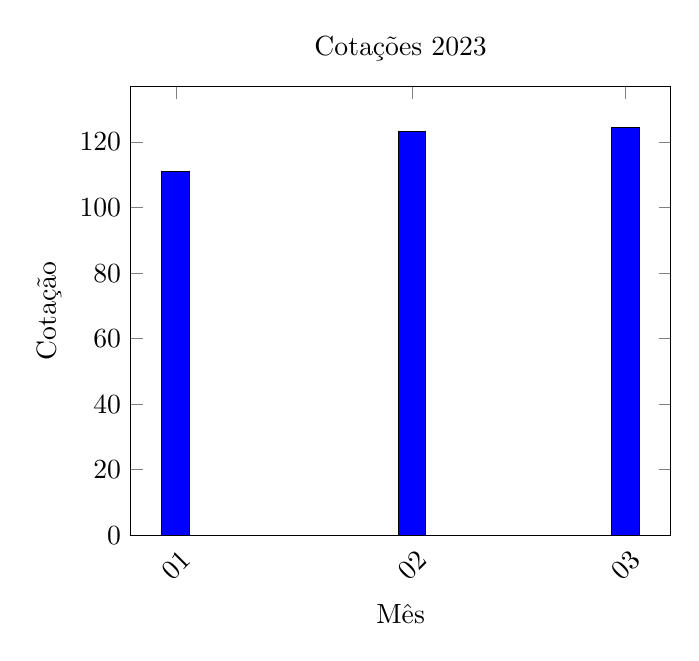
\begin{tikzpicture}
        \begin{axis}[
            title={Cotações 2023},
            xlabel={Mês},
            ylabel={Cotação},
            ymin=0,
            yticklabel style={
                /pgf/number format/fixed,
                /pgf/number format/precision=3
            },
            date coordinates in=x,
            xticklabel={\month},
            xtick={
                {2023-01-01},
                {2023-02-01},
                {2023-03-01},
                {2023-04-01}
            },
            xticklabel style={rotate=45, anchor=near xticklabel},
            ]
            \addplot[ybar,fill=blue] coordinates {
                (2023-01-01, 111.110)
                (2023-02-01, 123.280)
                (2023-03-01, 124.400)};
    \end{axis}
    \end{tikzpicture}
    \end{figure}

Com base nos dados apresentados no gráfico, é possível realizar uma análise dos dados do ano de 2021 até 2023, fornecendo uma visão abrangente do desempenho da Airbnb nesse período. Posteriormente, farei uma análise geral que engloba todo o período e destaca os principais insights.

    \section*{Análise dos Dados de 2021 a 2023:}

 Durante o período de 2021 a 2023, as cotações de mercado da Airbnb mostraram uma tendência ascendente, indicando um crescimento constante da empresa. No início de 2021, as ações da Airbnb ultrapassaram a marca dos 200 dólares, refletindo uma recuperação significativa em relação ao valor mínimo alcançado no final de 2020. A partir desse ponto, as cotações continuaram a subir ao longo de 2021, atingindo cerca de 166,5 dólares no final do ano.

 Em 2022, as cotações de mercado da Airbnb mantiveram-se relativamente estáveis nos primeiros meses, indicando uma consolidação do crescimento alcançado no ano anterior. No entanto, a partir de maio de 2022, as cotações começaram a declinar, atingindo seu valor mínimo no final do ano, em torno de 85,50 dólares por ação. Esse declínio pode ser atribuído a uma série de fatores, como a persistência da pandemia de COVID-19 e a concorrência acirrada no mercado de aluguel de curto prazo.

    \section*{Análise Geral:}

Ao realizar uma análise geral dos dados de 2021 a 2023, é evidente que a Airbnb passou por um período desafiador com a chegada da pandemia de COVID-19, que impactou negativamente o setor de turismo como um todo. No entanto, a empresa demonstrou resiliência ao adaptar-se às mudanças na demanda do mercado e conseguiu se recuperar em 2021, alcançando cotações de mercado significativamente mais altas do que no ano anterior.

Embora o desempenho da Airbnb tenha sido impactado negativamente em 2022, com uma queda acentuada nas cotações de mercado, é importante ressaltar que a empresa enfrentou desafios significativos durante esse período, como a persistência da pandemia e a competição acirrada. Esses fatores podem ter influenciado as expectativas dos investidores em relação ao desempenho futuro da empresa.

No entanto, é importante observar que os dados mais recentes de 2023 indicam uma trajetória ascendente nas cotações de mercado da Airbnb, sugerindo uma recuperação gradual. Essa recuperação pode ser atribuída à diminuição dos casos de COVID-19 globalmente e ao aumento da demanda por acomodações de viagem. Esses dados sugerem que a empresa continua a ser uma forte concorrente no mercado de compartilhamento de casas.

Em uma análise geral, podemos destacar a capacidade da Airbnb de se adaptar às mudanças do mercado, sua resiliência diante de desafios significativos e sua habilidade em se recuperar e manter uma trajetória ascendente em longo prazo. No entanto, é essencial considerar que o mercado financeiro é volátil.

    \section*{Como a Airbnb se encontra atualmente:}
A Airbnb está em uma posição sólida atualmente, como evidenciado pelos seus resultados financeiros do primeiro trimestre de 2023. A empresa registrou um recorde de receita de US\$ 1,8 bilhão, com um crescimento de 20\% em relação ao ano anterior. Além disso, alcançou seu primeiro trimestre lucrativo, com um lucro líquido de US\$ 117 milhões. O EBITDA ajustado foi de US\$ 262 milhões, um recorde no primeiro trimestre, e o fluxo de caixa livre atingiu US\$ 1,6 bilhão, o maior valor já registrado.

A Airbnb também apresentou um desempenho sólido em seu negócio principal. As noites e experiências reservadas aumentaram 19\% em comparação com o ano anterior, indicando uma base crescente de hóspedes fiéis e reservas de primeira viagem. O crescimento das reservas internacionais e a recuperação contínua da Ásia-Pacífico foram pontos positivos. A empresa também se destacou no segmento de estadias de longa duração, representando 18\% do total de noites brutas reservadas.

Além disso, a Airbnb continua focada em suas prioridades estratégicas, como tornar a hospedagem mainstream, aperfeiçoar o serviço principal e expandir além do núcleo. A empresa investe em conscientização, facilidade de uso e melhoria do serviço por meio de novos recursos e atualizações. Seus esforços resultam em um crescimento consistente das listagens ativas.

No geral, a Airbnb se encontra em uma posição favorável, com resultados financeiros positivos, crescimento da oferta, expansão internacional e satisfação dos hóspedes. A empresa continua aprimorando sua plataforma e explorando novas oportunidades para manter sua liderança no mercado de hospedagem.
% -------------------------%
    \section*{O que esperar do futuro da Airbnb?}
O futuro da Airbnb parece promissor, apesar dos desafios enfrentados. A empresa revolucionou o setor de hospitalidade ao conectar viajantes com anfitriões que desejam alugar suas propriedades. Mesmo durante a pandemia, a demanda por aluguéis de curta duração aumentou, impulsionada pelo desejo de liberdade dos viajantes e pela busca por acomodações mais acessíveis. A Airbnb registrou um aumento significativo no número de listagens nos Estados Unidos, indicando um mercado competitivo para os anfitriões. No entanto, a empresa conseguiu obter resultados financeiros positivos, relatando vendas recordes e demonstrando sua capacidade de se adaptar às mudanças na demanda.

Para o futuro, a Airbnb está focada em investir em projetos de capital e continuar aprimorando seu modelo de negócio. A empresa tem mostrado sua capacidade de transformar receita em fluxo de caixa, mantendo uma margem de fluxo de caixa livre de mais de 40\%. Além disso, a Airbnb possui uma posição de destaque no mercado de viagens, com potencial para expandir sua participação e aumentar suas margens de lucro. A empresa está se adaptando ao aumento do trabalho remoto e às mudanças nas preferências dos viajantes, garantindo que continue a ser uma força disruptiva no setor.

Embora os desafios persistam, como o mercado competitivo de aluguéis de curta duração e a possibilidade de falência, a Airbnb demonstrou resiliência e capacidade de ajustar-se às demandas em constante mudança. Com uma base sólida de usuários e uma proposta de valor única, a empresa está bem posicionada para enfrentar os desafios futuros e continuar a crescer. Os investidores podem considerar a Airbnb como uma opção atraente, pois a empresa possui um potencial de mercado significativo e está em um estágio de crescimento acelerado.
\newpage
% -------------------------%
    \section*{Metodologia}
Neste estudo, foram utilizadas duas ferramentas de busca na internet, o Chat do Bing e o Google, para realizar pesquisas rápidas e obter informações relevantes sobre a empresa Airbnb e suas cotações de mercado.

A primeira etapa da metodologia consistiu em utilizar o Chat do Bing para acessar informações específicas sobre a Airbnb, como seu desempenho financeiro, impacto da pandemia de COVID-19 e estratégias de recuperação adotadas pela empresa. Essa ferramenta de busca foi escolhida devido à sua interface interativa, que permite realizar consultas e obter respostas de forma ágil.

Em seguida, o Google foi utilizado para aprofundar a pesquisa e obter informações adicionais sobre a Airbnb, como notícias recentes, análises de mercado e tendências do setor de turismo. O Google é uma ferramenta amplamente utilizada e fornece resultados de busca abrangentes e atualizados.

Além disso, os dados utilizados para construir os gráficos de cotações de mercado da Airbnb foram obtidos no Yahoo Finances. Essa plataforma online é reconhecida por disponibilizar informações financeiras e histórico de cotações de ações de diversas empresas. Os dados foram coletados para os anos de 2021, 2022 e 2023, permitindo uma análise longitudinal do desempenho da Airbnb.

Após a coleta dos dados, eles foram tabulados e analisados quantitativamente. Os gráficos foram construídos utilizando o LaTex Workshop, um software de visualização de dados amplamente utilizado para criação de documentos científicos. Essa ferramenta oferece recursos avançados de formatação e geração de gráficos de alta qualidade, garantindo a clareza e a legibilidade das informações apresentadas.

É importante ressaltar que todas as informações coletadas e utilizadas neste estudo são de fontes públicas disponíveis na internet, e a precisão e veracidade dos dados dependem da confiabilidade dessas fontes.

Por fim, é fundamental destacar que essa metodologia foi adotada como uma abordagem para a coleta de dados e análise do desempenho da Airbnb. Outras metodologias podem ser utilizadas em estudos futuros para uma análise mais aprofundada e abrangente.

Ao seguir essa metodologia, buscamos garantir a obtenção de informações confiáveis e a realização de uma análise rigorosa do desempenho da Airbnb no período de 2021 a 2023. As etapas descritas acima foram fundamentais para uma análise abrangente e embasada, contribuindo para a compreensão do cenário atual da Airbnb e suas perspectivas futuras.
% -------------------------%
\newpage
\section*{Conclusão}
A pandemia de COVID-19 8 teve um impacto significativo no setor de viagens e no Airbnb, apresentando desafios e exigindo adaptações por parte da empresa. Durante esse período, houve uma redução drástica das viagens, cancelamentos em massa, mudança para estadias de longa duração e a necessidade de implementar medidas de limpeza e segurança mais rigorosas. No entanto, o Airbnb demonstrou resiliência ao implementar estratégias como o foco em viagens domésticas, experiências locais e aprimoramento das medidas de segurança e higiene.

Apesar das dificuldades enfrentadas, o Airbnb atualmente se encontra em uma posição sólida no mercado. Os resultados financeiros do primeiro trimestre de 2023 indicam um crescimento notável, com um aumento de 20\% na receita em relação ao ano anterior, alcançando um trimestre lucrativo com um lucro líquido de 177 milhões. Além disso, o número de noites e experiências reservadas também apresentou um aumento de 19\% em comparação ao ano anterior.

O Airbnb revolucionou o setor de hospedagem ao adotar um modelo de negócio inovador, conectando viajantes a anfitriões que desejam alugar suas propriedades. Durante a pandemia, a empresa demonstrou sua capacidade de adaptação, lançando novas iniciativas, como experiências virtuais, estadias flexíveis e reservas de longo prazo, para atender às necessidades dos usuários em meio à crise.

Olhando para o futuro, o Airbnb tem uma perspectiva promissora. A empresa está empenhada em investir em projetos de capital e continuar aprimorando seu modelo de negócio. Com sua posição consolidada no mercado e sua capacidade de inovação, o Airbnb está bem posicionado para enfrentar os desafios futuros e aproveitar as oportunidades no setor de hospedagem.

Em suma, a pandemia de COVID-19 impactou o Airbnb de diversas maneiras, mas a empresa mostrou resiliência ao adaptar-se às novas demandas do mercado. Com sua posição sólida, crescimento financeiro e capacidade de inovação, o Airbnb está preparado para enfrentar o futuro com confiança e continuar a oferecer uma experiência diferenciada aos viajantes e anfitriões.
\newpage
\section*{Referências}
\bibitem{airbnb_limpeza1}
Airbnb. \textit{Guia de início rápido de limpeza}. Disponível em: \url{https://assets.contentstack.io/v3/assets/bltb428ce5d46f8efd8/bltff19165e9317c088/5ee8249ddaf3a20c35d1191f/CleaningQuickStart_PT_BR.pdf}

\bibitem{airbnb_saude}
Airbnb. \textit{Saúde e segurança na pandemia}. Disponível em: \url{https://news.airbnb.com/br/saude-e-seguranca-na-pandemia/}

\bibitem{veja_airbnb}
Veja. \textit{Airbnb na pandemia: da hora mais escura aos planos de IPO nos EUA}. Disponível em: \url{https://veja.abril.com.br/economia/airbnb-na-pandemia-da-hora-mais-escura-aos-planos-de-ipo-nos-eua/}

\bibitem{linkedin_airbnb}
Silva, M. A. \textit{Qual é o modelo de negócios por trás do Airbnb?}. Disponível em: \url{https://www.linkedin.com/pulse/qual-\%C3\%A9-o-modelo-de-neg\%C3\%B3cios-por-tr\%C3\%A1s-do-airbnb-marco-antonio-da-silva/?originalSubdomain=pt}

\bibitem{uol_airbnb}
UOL. \textit{Turismo pós-covid: “Na crise, seremos parte da solução", diz CEO do Airbnb}. Disponível em: \url{https://www.uol.com.br/nossa/reportagens-especiais/turismo-pos-covid-na-crise-seremos-parte-da-solucao-diz-ceo-do-airbnb/#page1}

\bibitem{artigo_airbnb}
Cruz, P., Ribeiro, F., & Machado, V. (2021). \textit{A percepção dos consumidores acerca do uso do Airbnb durante a pandemia de Covid-19}. Disponível em: \url{https://repositorium.sdum.uminho.pt/handle/1822/73704}

\bibitem{USP_airbnb}
USP. \textit{Impactos da pandemia no setor de turismo}. Disponível em: \url{https://jornal.usp.br/artigos/impactos-da-pandemia-no-setor-de-turismo/}

Airbnb. \textit{Airbnb apresenta um programa de limpeza avançada para o futuro das viagens}. Disponível em: \url{https://news.airbnb.com/pt/airbnb-apresenta-um-programa-de-limpeza-avancada-para-o-futuro-das-viagens/}. 

\bibitem{airbnb_limpeza2}
Airbnb. \textit{Airbnb anuncia o protocolo de limpeza avançada}. Disponível em: \url{https://news.airbnb.com/pt/airbnb-apresenta-um-programa-de-limpeza-avancada-para-o-futuro-das-viagens/}. 

\bibitem{airbnb_covid1}
Airbnb. \textit{Protocolos de segurança e higiene da Airbnb para ajudar a prevenir a propagação da COVID-19}. Disponível em: \url{https://www.airbnb.com.br/help/article/2728}. 

\bibitem{airbnb_covid2}
Airbnb. \textit{Recursos de segurança COVID-19}. Disponível em: \url{https://www.airbnb.com.br/d/covidsafety}

\bibitem{airbnb_covid3}
Airbnb. \textit{COVID-19 e seu negócio de hospedagem: como minimizar o impacto}. Disponível em: \url{https://www.airbnb.com.br/resources/hosting-homes/a/covid-19-your-hosting-business-how-to-minimize-the-impact-152}

\bibitem{airbnb_covid_protocolos}
Airbnb. \textit{Protocolos de segurança e higiene da Airbnb para ajudar a prevenir a propagação da COVID-19}. Disponível em: \url{https://www.airbnb.com.br/help/article/2728}.

\bibitem{airbnb_vizinho}
Airbnb. \textit{Airbnb lança canal de apoio ao vizinho no Brasil para auxiliar as cidades}. Disponível em: \url{https://news.airbnb.com/br/airbnb-lanca-canal-de-apoio-ao-vizinho-no-brasil-para-auxiliar-as-cidades/}.

\bibitem{airbnb_vizinho_forum}
Airbnb. \textit{Canal de Apoio ao Vizinho no Brasil}. Disponível em: \url{https://community.withairbnb.com/t5/Ajuda/Canal-de-Apoio-ao-Vizinho-no-Brasil/m-p/1442756}.

\bibitem{airbnb_pandemic}
Frenkel, Sheera. \textit{Airbnb’s Business Was Booming. Then the Pandemic Hit}. Disponível em: \url{https://www.nytimes.com/2020/09/24/travel/airbnb-pandemic.html}.

\bibitem{yahoo_finances}
Yahoo Finanças. Disponível em: \url{https://br.financas.yahoo.com}.

\bibite{Discontinued News}
Discontinued News. Disponível em: \url{https://discontinuednews.com/is-airbnb-going-out-of-business/#:~:text=After\%20a\%20strong\%20year\%20in\%202022\%2C\%20Airbnb\%E2\%80\%99s\%20growth,time\%2C\%20there\%20are\%20no\%20layoffs\%20at\%20the\%20company.}
\end{document}